\documentclass[tikz,border=10pt]{standalone}
\usepackage{tikz}
\usetikzlibrary{positioning,shapes.geometric,arrows.meta,calc}

% Using hexagon tessellation approach based on tikz-hexagon library
% Reference: https://github.com/mossblaser/tikz-hexagon

\begin{document}
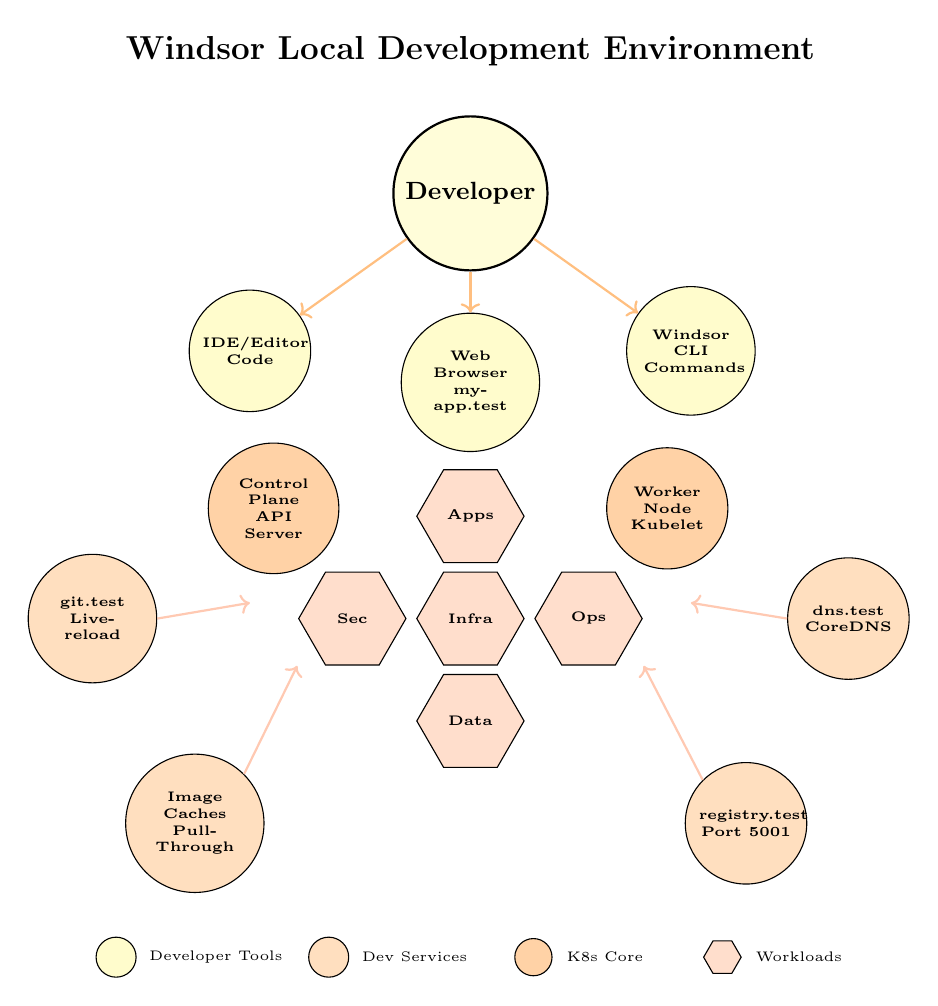
\begin{tikzpicture}[
    % Node styles with muted yellow/gold to burnt orange/red spectrum
    developer/.style={circle, draw=black, thick, fill=yellow!15!white, minimum size=1.5cm, font=\small\bfseries},
    tool/.style={circle, draw=black, fill=yellow!20!white, minimum size=1.4cm, font=\tiny\bfseries, text width=1.2cm, align=center},
    service/.style={circle, draw=black, fill=orange!25!white, minimum size=1.4cm, font=\tiny\bfseries, text width=1.2cm, align=center},
    k8s-core/.style={circle, draw=black, fill=orange!35!white, minimum size=1.3cm, font=\tiny\bfseries, text width=1.1cm, align=center},
    k8s-inner/.style={regular polygon, regular polygon sides=6, draw=black, fill=red!30!orange!20!white, minimum size=0.8cm, text width=0.6cm, align=center, font=\tiny\bfseries},
    % Arrow styles
    connection/.style={->, orange!50, thick},
    % Text styles
    title/.style={font=\large\bfseries}
]

% Title
\node[title] at (0, 8) {Windsor Local Development Environment};

% Central core - Developer at top (moved up)
\node[developer] (dev) at (0, 6.2) {Developer};

% Inner ring - Developer Tools (better spacing)
\node[tool] (ide) at (-2.8, 4.2) {IDE/Editor\\{\tiny Code}};
\node[tool] (browser) at (0, 3.8) {Web Browser\\{\tiny my-app.test}};
\node[tool] (cli) at (2.8, 4.2) {Windsor CLI\\{\tiny Commands}};

% Middle ring - K8s Core Components (better positioned)
\node[k8s-core] (control) at (-2.5, 2.2) {Control\\Plane\\{\tiny API Server}};
\node[k8s-core] (worker) at (2.5, 2.2) {Worker\\Node\\{\tiny Kubelet}};

% Central hexagonal cluster - Infra-centered arrangement with better spacing
% Infra at center with others positioned around it
% Apps top, Data bottom, Sec left, Ops right - increased horizontal spacing

\node[k8s-inner] (infra) at (0, 0.8) {Infra};         % Center - Infra now central
\node[k8s-inner] (apps) at (0, 2.1) {Apps};           % Top - Apps moved up
\node[k8s-inner] (data) at (0, -0.5) {Data};          % Bottom - Data moved down
\node[k8s-inner] (services) at (-1.5, 0.8) {Sec};     % Left - increased spacing
\node[k8s-inner] (ops) at (1.5, 0.8) {Ops};           % Right - increased spacing

% Outer ring - Infrastructure Services (better spacing)
\node[service] (git) at (-4.8, 0.8) {git.test\\{\tiny Live-reload}};
\node[service] (dns) at (4.8, 0.8) {dns.test\\{\tiny CoreDNS}};
\node[service] (cache) at (-3.5, -1.8) {Image\\Caches\\{\tiny Pull-Through}};
\node[service] (registry) at (3.5, -1.8) {registry.test\\{\tiny Port 5001}};

% Connections from Developer to tools (clean radial lines)
\draw[connection] (dev) -- (ide);
\draw[connection] (dev) -- (browser);
\draw[connection] (dev) -- (cli);

    % General inward flow - outer services pointing vaguely toward Infra area (shortened)
    \draw[->, red!40!orange!30, thick] (git.east) -- (-2.8, 1.0);
    \draw[->, red!40!orange!30, thick] (dns.west) -- (2.8, 1.0);
    \draw[->, red!40!orange!30, thick] (cache.north east) -- (-2.2, 0.2);
    \draw[->, red!40!orange!30, thick] (registry.north west) -- (2.2, 0.2);

% Legend - positioned below and centered with better spacing
\begin{scope}[shift={(0,-3.5)}]
    \node[tool, scale=0.35] at (-4.5,0) {};
    \node[right, font=\tiny] at (-4.2,0) {Developer Tools};

    \node[service, scale=0.35] at (-1.8,0) {};
    \node[right, font=\tiny] at (-1.5,0) {Dev Services};

    \node[k8s-core, scale=0.35] at (0.8,0) {};
    \node[right, font=\tiny] at (1.1,0) {K8s Core};

    \node[k8s-inner, scale=0.35] at (3.2,0) {};
    \node[right, font=\tiny] at (3.5,0) {Workloads};
\end{scope}

\end{tikzpicture}
\end{document}
